\clearpage
\part{Temporal, Geometric, Multi-Horizon, and Causal Extensions}

\section{Next-onset forecasts}
Accessible volume can be moved from token identity to time only when a model supplies a normalized distribution over a finite timing vocabulary. Let $H_i$ be the musical history before event $i$ and define
\begin{equation}
\mathcal O_\delta=\{\delta,2\delta,\ldots,M\delta\},\qquad
p_i(k)=P(\text{next onset occurs after }k\delta\mid H_i).
\end{equation}
The next-onset count is
\begin{equation}
A_{\tau,i}(H_i)=\sum_{k=1}^{M}\indicator[p_i(k)>\tau].
\label{eq:onset-volume}
\end{equation}
A tempo-independent representation normalizes intervals by seconds per beat $B$:
\begin{equation}
r_i=\frac{t_{i+1}-t_i}{B},\qquad p_i(k)=P(r_i\in I_k\mid H_i),
\label{eq:normalized-interval}
\end{equation}
where $I_k$ are declared interval bins. The result is a property of the model, history, quantization, and threshold, not an intrinsic uncertainty possessed by a song or listener.

Timing correctness remains separate. For predicted onset $\hat t_i$ and observed onset $t_i$,
\begin{equation}
e_i=t_i-\hat t_i,\qquad
E_{\mathrm{RMSE}}=\sqrt{\frac1n\sum_{i=1}^{n}(t_i-\hat t_i)^2}.
\label{eq:timing-error}
\end{equation}
A present-state record can preserve breadth, momentum, and error without combining incompatible units:
\begin{equation}
\mathcal S_i=(A_{\tau,i}(H_i),M_{\tau,i},e_i),\qquad
M_{\tau,i}=A_{\tau,i}(H_i)-A_{\tau,i-1}(H_{i-1}).
\end{equation}
A separate controller could use
\begin{equation}
a_{i+1}=\pi(\mathcal S_i,\text{candidates}_i,\text{goal},\text{constraints}).
\label{eq:temporal-control}
\end{equation}
Equation~\eqref{eq:temporal-control} is a control hypothesis. Accessible volume supplies neither a reward nor a direction; goals, candidate semantics, and observed outcomes remain necessary.

\section{Geometric comparison and temporal reflection}
For corresponding one-dimensional onset vectors, restricted Procrustes alignment fits
\begin{equation}
q_i\approx ap_i+b,\qquad a>0,
\end{equation}
where $a$ removes tempo scale and $b$ starting position. The residual is
\begin{equation}
D(p,q)=\sqrt{\frac1n\sum_{i=1}^{n}\bigl(q_i-(ap_i+b)\bigr)^2}.
\label{eq:procrustes-1d}
\end{equation}
Temporal reflection for sequence length $L$ produces $p'_i=L-p_{n+1-i}$, followed by reordering, and
\begin{equation}
D_{\mathrm{retrograde}}=D(p,p').
\end{equation}
A zero residual means exact agreement after this restricted alignment. It does not imply musical, causal, or semantic identity. At least three onsets are needed for a nontrivial structural comparison because two distinct pairs can always be aligned by scale and translation. The Groove implementation uses nonnegative scale and records degenerate scales; no degeneracy occurred in the reported test set. The full two-dimensional similarity, rigid, and affine formulations are collected in Appendix~\ref{app:geometry-equations}.

\section{Synthetic rhythm experiment}
\subsection{Method}
The synthetic study used eight motifs with 60 training and 20 held-out variations per motif. Tempo ranged from 65 to 150 beats per minute and intervals received Gaussian jitter with standard deviation 0.025 beats. Held-out variations shared their underlying motifs with training, so the experiment did not test unseen-motif generalization.

The pipeline normalized intervals by seconds per beat, centered and unit-scaled trailing four-interval onset vectors, fitted eight $k$-means context clusters on training windows only, and trained a hierarchically smoothed categorical predictor using context cluster and the previous two interval bins. The target vocabulary had eight interval categories and smoothing $\alpha=4$. Accessible volume was evaluated over 100 thresholds from $0.005$ to $0.5$. Forward-trained prediction was evaluated on forward and reversed held-out sequences.

\subsection{Results}
\begin{table}[htbp]
\centering
\caption{Synthetic next-onset results. Mean $A$ averages over the 100-threshold sweep.}
\label{tab:synthetic}
\begin{tabular}{lrrrrr}
\toprule
Condition&Top-1&Log-loss&Mean max $p$&Mean $A$&Sweep area\\
\midrule
Forward&\textbf{84.4\%}&\textbf{0.339}&0.842&1.31&0.647\\
Retrograde&59.0\%&2.899&0.839&1.31&0.649\\
\bottomrule
\end{tabular}
\end{table}
The exact seeded implementation produced 1,620 correct forward and 1,132 correct retrograde predictions among 1,920 per condition: 84.375\% and 58.958\%. Log-loss values were 0.338856 and 2.898662, with sweep areas 0.647474 and 0.649180. A deterministic linear-extrapolation baseline achieved 37.019\% forward and 32.837\% retrograde but supplied no probability distribution and therefore no accessible volume.

\begin{figure}[htbp]
\centering
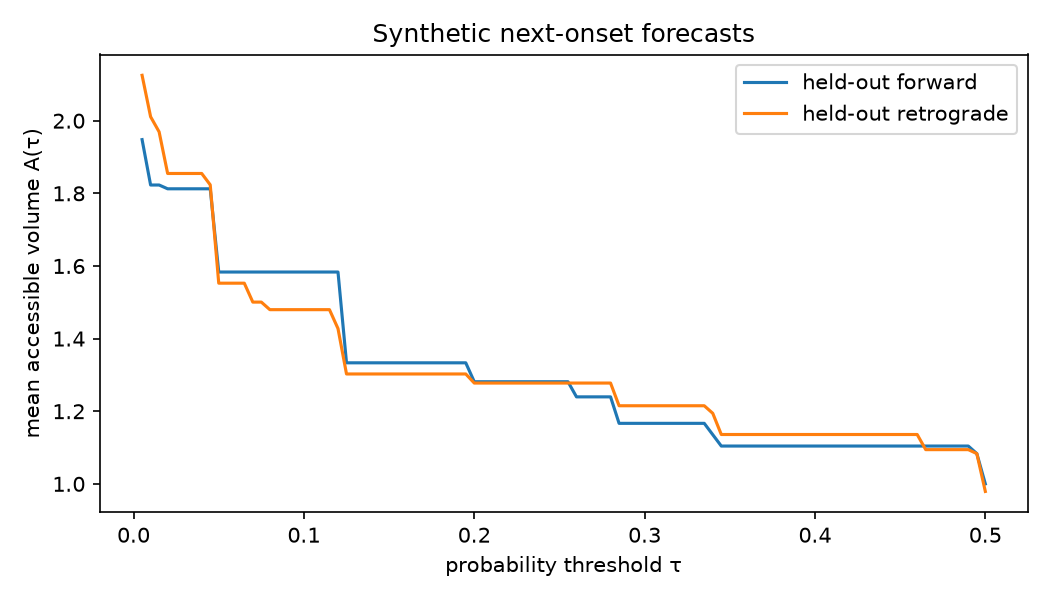
\includegraphics[width=0.9\textwidth]{rhythm-synthetic.png}
\caption{Synthetic forward and retrograde accessible-volume sweeps. Similar breadth coexists with substantially different correctness and log-loss.}
\label{fig:synthetic}
\end{figure}
Reversal reduced top-1 by 25.4 percentage points and greatly increased log-loss while mean accessible volume remained unchanged to two decimal places. Mean maximum probability also remained close. The retrograde predictor was often confidently wrong. This is a direct empirical separation of breadth, confidence, and correctness.

\section{Magenta Groove human-drumming experiment}
\subsection{Data and matched reversal control}
The real-MIDI study used Magenta Groove MIDI Dataset v1.0.0, licensed CC BY 4.0 \cite{magentagroove}. The source manifest covers 514 usable 4/4 performances. Grouped splitting by recording session produced 396 training and 118 held-out performances with zero session overlap. The official split was not used because 17 sessions crossed its train/test boundary. Splitting preceded context clustering and window training.

Only drum-channel onsets were used. Onsets separated by at most 0.02 quarter-note beats were merged. Intervals remained in MIDI beat units, cancelling tempo. Targets used 48 bins per beat up to four beats, producing 192 categories. Each context contained four trailing intervals and one of 16 training-fitted clusters. The categorical predictor used the previous two bins and hierarchical smoothing with $\alpha=4$. Training produced 218,033 windows; every condition evaluated 121,392 held-out predictions.

Three conditions were distinguished:
\begin{itemize}
  \item \textbf{Forward:} forward training and forward evaluation.
  \item \textbf{Reversal transfer:} the forward model evaluated on reversed held-out performances with forward-fitted clusters.
  \item \textbf{Backward matched:} the same architecture and count-table procedure trained on reversed training performances and evaluated on reversed test performances.
\end{itemize}
The backward-matched condition separates a model-transfer penalty from the learnability of reversed structure.

\subsection{Results}
\begin{table}[htbp]
\centering
\caption{Magenta Groove results over 121,392 predictions per condition.}
\label{tab:groove}
{\small
\setlength{\tabcolsep}{4pt}
\begin{tabular}{lrrrrrr}
\toprule
Condition&Top-1&Top-5&Log-loss&ECE&Mean $A$&Sweep area\\
\midrule
Forward&\textbf{17.33\%}&\textbf{56.12\%}&3.194&0.060&1.886&0.899\\
Reversal transfer&16.01\%&52.99\%&3.333&0.072&1.885&0.898\\
Backward matched&17.06\%&55.52\%&\textbf{3.183}&0.060&1.886&0.899\\
\bottomrule
\end{tabular}}
\end{table}
The backward-matched model nearly recovered forward top-1 and top-5 performance and had numerically slightly lower log-loss. No significance test is claimed for that small difference. Direct reversal transfer performed worse. The supported conclusion is that reversed rhythms are learnable by the same model class, not that time reversal has no effect in every system.

Mean maximum probabilities were 0.233 forward, 0.232 for reversal transfer, and 0.230 for backward matching. Mean accessible volume and sweep area again changed only slightly while accuracy and log-loss varied. Low top-1 is expected for fine-grained human timing over 192 categories and must not be compared directly with the eight-category synthetic task.

\begin{figure}[htbp]
\centering
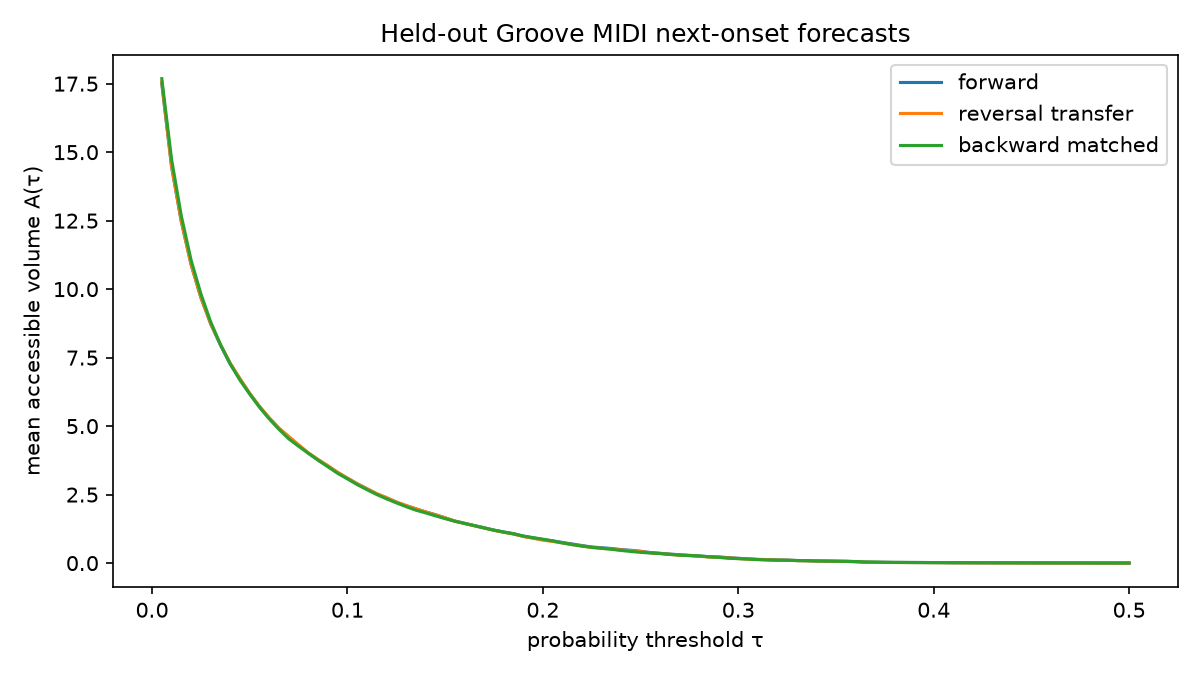
\includegraphics[width=0.95\textwidth]{groove-accessible-volume.png}
\caption{Groove sweeps for forward, reversal-transfer, and backward-matched conditions.}
\label{fig:groove-sweep}
\end{figure}
\begin{figure}[htbp]
\centering
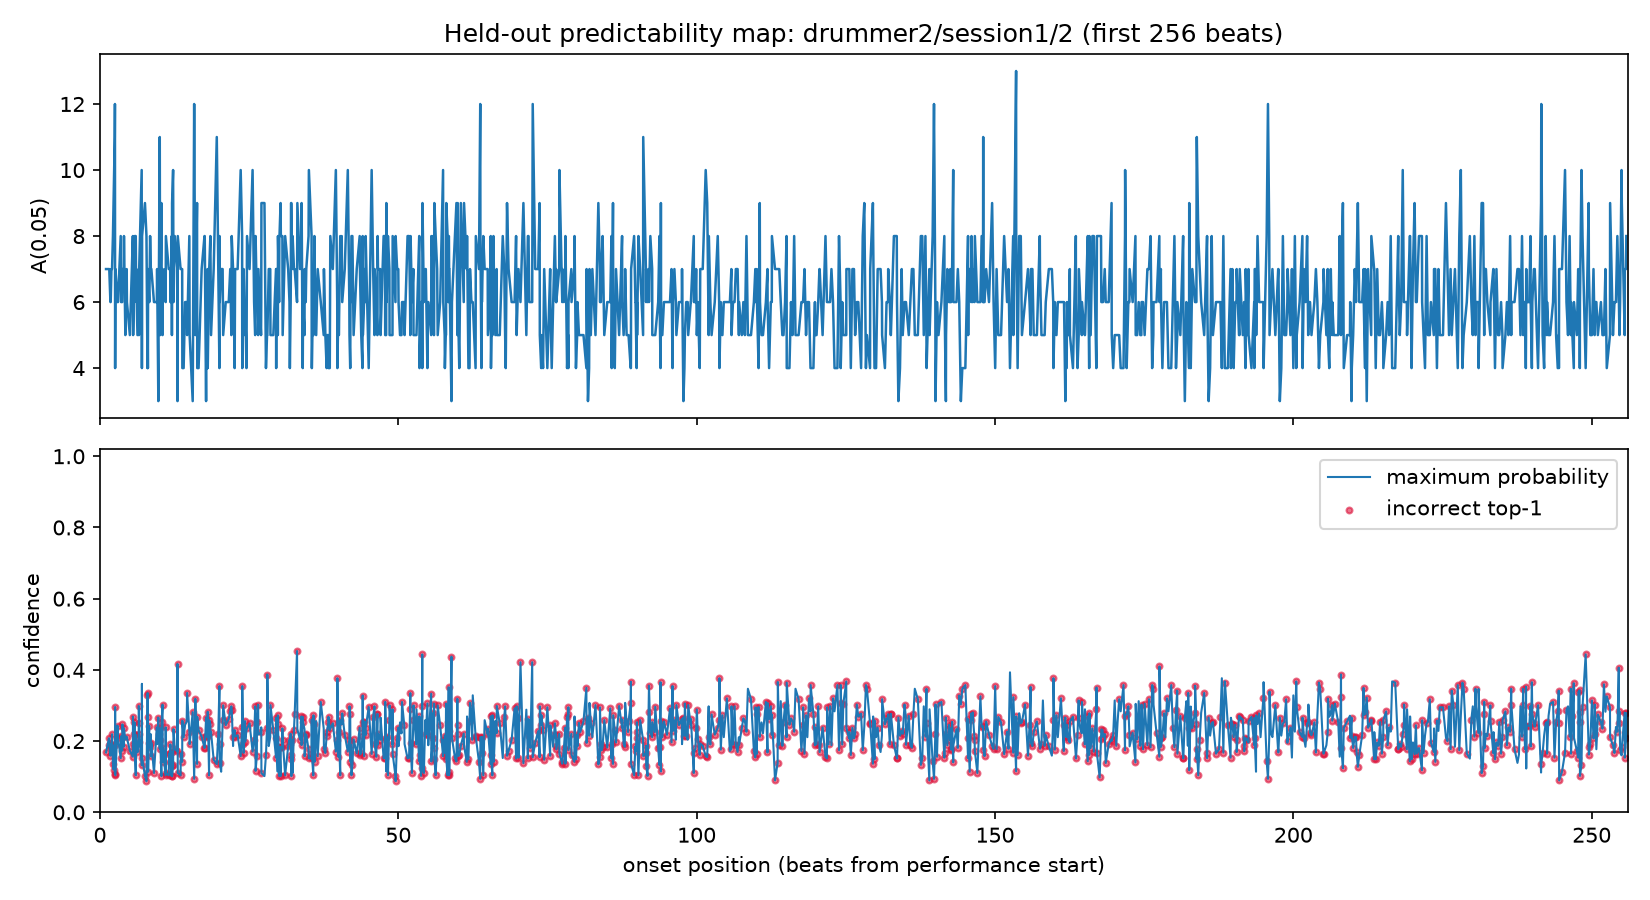
\includegraphics[width=0.97\textwidth]{groove-predictability-map.png}
\caption{Accessible volume, confidence, and incorrect predictions over the first 256 beats of a held-out Groove performance. Breadth and correctness are displayed together rather than collapsed.}
\label{fig:groove-map}
\end{figure}

Procrustes alignment was also applied to each held-out performance and its reversed interval sequence. Across 118 performances, mean RMS residual was 5.633 beats, median 2.557 beats, and mean normalized residual 0.06252. No degenerate scale occurred. These residuals describe geometric dissimilarity after alignment; they do not explain correctness.

The saved NPZ preserves independent probability arrays, targets, sequence indices, and target positions for all three conditions. Independent recomputation checked headline metrics, fixed-threshold counts, source and artifact hashes, and the disjoint session split. Two complete runs produced identical numerical results.

\section{Nightingale classical, jazz, and folk experiment}
The second real-MIDI study used 140 usable files per genre from the Nightingale MIDI repository \cite{nightingale}. After deterministic shuffling, 100 files per genre were used for training and 40 for testing, yielding 420 files. Unlike Groove, this was a file-level split and lacked a separately trained backward-matched condition.

Parsing merged simultaneous onsets, converted ticks to beats, retained the longest segment with at least 64 positive intervals, and used at most 512 intervals. Gaps over eight beats separated segments. Thirteen interval categories, 24 context clusters, four trailing intervals, and smoothing $\alpha=4$ defined the shared model. Training used 139,839 onset positions and evaluation 57,113 predictions per direction.
\begin{table}[htbp]
\centering
\caption{Nightingale results. F/R denotes forward/retrograde; $N$ is per direction.}
\label{tab:nightingale}
{\scriptsize
\setlength{\tabcolsep}{3.5pt}
\begin{tabular}{lrrrrrr}
\toprule
Genre&$N$&Top-1 F/R&Log-loss F/R&$A_{0.1}$ F/R&Persistence F&ECE F\\
\midrule
Classical&17,276&68.3\%/67.9\%&0.976/1.024&1.91/1.91&66.7\%&0.064\\
Jazz&20,075&49.5\%/47.1\%&1.474/1.528&2.69/2.64&39.3\%&0.049\\
Folk&19,762&61.9\%/61.4\%&1.125/1.143&2.21/2.22&54.8\%&0.031\\
\bottomrule
\end{tabular}}
\end{table}
Under this model and quantization, jazz had the lowest top-1, highest log-loss, and broadest forecasts; classical had the narrowest and most accurate. The categorical predictor exceeded persistence in every genre. Retrograde changes were small in this transfer setup, which does not contradict Groove because the datasets, representations, and controls differ. The defensible joint conclusion is that reversal has no universal predictability direction independent of model and training.

\begin{figure}[htbp]
\centering
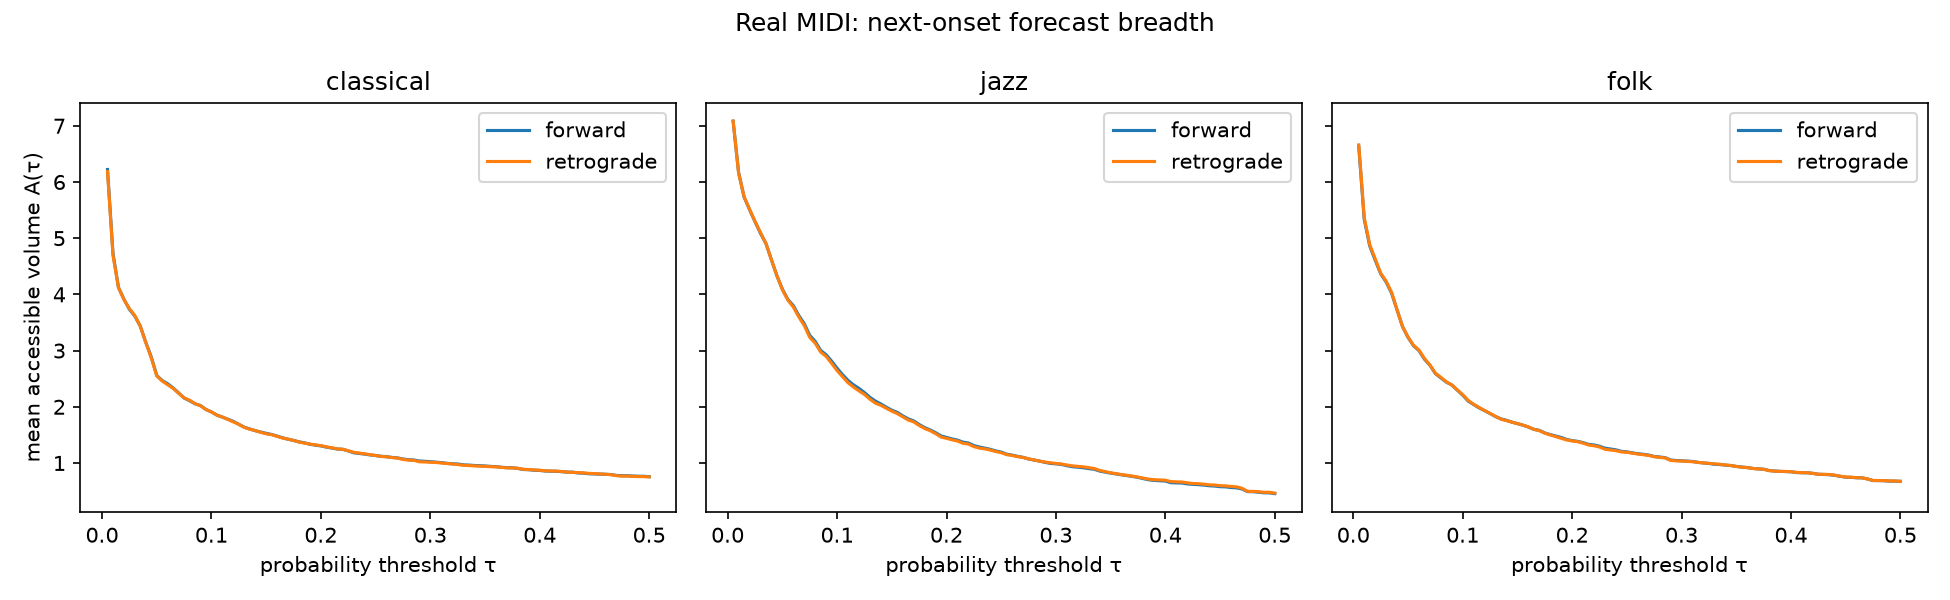
\includegraphics[width=0.97\textwidth]{nightingale-accessible-volume.png}
\caption{Nightingale accessible-volume sweeps by genre and direction.}
\label{fig:nightingale-sweep}
\end{figure}
\begin{figure}[htbp]
\centering
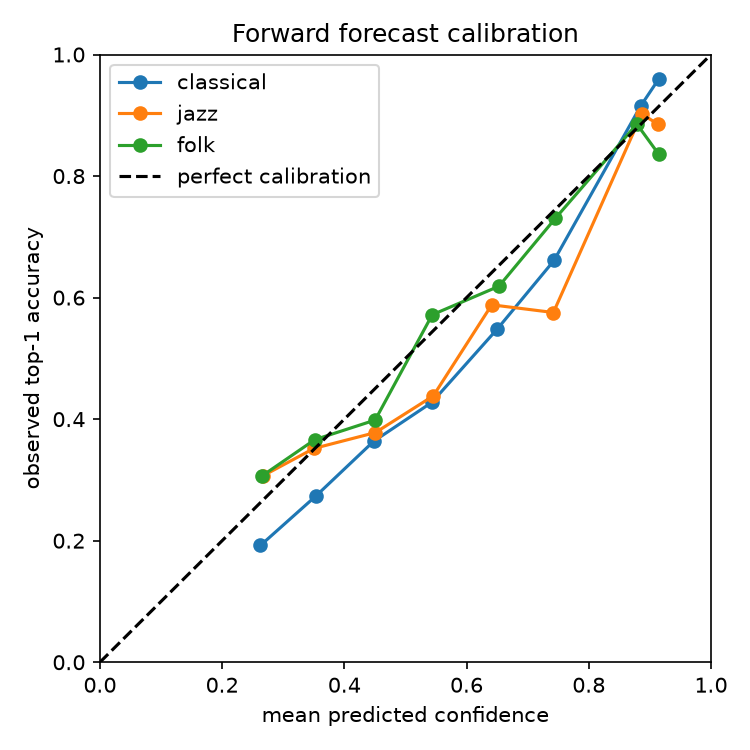
\includegraphics[width=0.66\textwidth]{nightingale-calibration.png}
\caption{Forward forecast calibration for the three Nightingale genres.}
\label{fig:nightingale-calibration}
\end{figure}

The repository also contains 18 listening excerpts stratified by genre and low, medium, or high $A_{0.1}$. Its browser interface requests a 1--5 surprise rating and exports data for Spearman correlations with accessible volume, entropy, negative log probability, and maximum probability. \textbf{No human correlation is reported}: real ratings remain pending and no synthetic judgments were substituted. Browser testing is interface validation, not perceptual evidence.

\section{HOP: a rejected geometric predictor}
The Harmonic Osculating Predictor (HOP) tested whether local hidden-state trajectories could be extrapolated as turning paths. The experiment evaluated 1,647 positions from extracted music-theory and classical-geometry chapters and repeated code using DistilGPT-2 \cite{distilgpt2}. Tokens were ranked through the learned output embedding, not an assumed cosine decoder.

Let $v_0=h_{t-1}-h_{t-2}$ and $v_1=h_t-h_{t-1}$. Define $u=v_0/\lVert v_0\rVert$ and let $w$ be the normalized component of $v_1$ orthogonal to $u$. The signed angle and implemented speed ratio are
\begin{equation}
\theta=\operatorname{atan2}(v_1\cdot w,v_1\cdot u),\qquad
s=\operatorname{clip}\!\left(\frac{\lVert v_1\rVert}{\lVert v_0\rVert},0.25,4\right).
\end{equation}
With $\Delta\theta$ estimated from the preceding turn when available and
$\phi_k=(k+2)\theta+k\Delta\theta$, the evaluated composed-rotation rule is
\begin{equation}
\hat h_{t+n}=h_t+\sum_{k=0}^{n-1}s^{k+1}\lVert v_1\rVert
\left[\cos(\phi_k)u+\sin(\phi_k)w\right].
\label{eq:hop}
\end{equation}
Degenerate vectors use source-defined linear fallbacks. Equation~\eqref{eq:hop} corrects an earlier non-accumulating expression that added the same rotated displacement repeatedly and could reduce to a straight line rather than an arc.
\begin{table}[htbp]
\centering
\caption{HOP and comparison predictors over 1,647 hidden-state positions.}
\label{tab:hop}
\begin{tabular}{lrr}
\toprule
Predictor&Top-1&Top-5\\
\midrule
Model, one ahead&\textbf{46.6\%}&\textbf{66.6\%}\\
Linear velocity, one ahead&41.3\%&60.0\%\\
HOP, one ahead&11.3\%&21.4\%\\
Repeat token, two ahead&\textbf{5.4\%}&5.4\%\\
Linear velocity, two ahead&5.0\%&\textbf{9.4\%}\\
HOP, two ahead&3.2\%&8.1\%\\
\bottomrule
\end{tabular}
\end{table}
HOP lost decisively. For this model and text sample, hidden states did not follow these turning paths often enough to outperform linear velocity. This is a negative result for the tested construction, not a theorem against all geometric prediction.

Several stronger interpretations are explicitly rejected: arbitrary states in $\mathbb R^d$ need not be collinear, so a four-point projective cross-ratio is not an established cadence detector; nonzero curvature alone does not imply error growth $\varepsilon e^{\kappa n}$; musical terms are metaphors unless independently operationalized; and learned multi-token systems such as Medusa or EAGLE do not validate this handcrafted rule. HOP supplies a point forecast, not a distribution, so it cannot supply accessible volume without separately calibrated and discretized errors.

\section{Multi-horizon accessible volume}
\subsection{Complete continuations}
Let $C_t$ be an autoregressive context and $a_{1:h}=(a_1,\ldots,a_h)$ a complete candidate continuation. The learned conditional joint probability is
\begin{equation}
P_h(a_{1:h}\mid C_t)=
\prod_{j=1}^{h}p(a_j\mid C_{t+j-1},a_{<j}),
\label{eq:joint-continuation}
\end{equation}
where each candidate prefix is carried into the next context. Multi-horizon accessible volume and its complement are
\begin{align}
A^{(h)}_\tau(C_t)&=\sum_{a_{1:h}\in\mathcal O^h}
\indicator[P_h(a_{1:h}\mid C_t)>\tau],\label{eq:multi-horizon}\\
A^{c,(h)}_\tau(C_t)&=|\mathcal O|^h-A^{(h)}_\tau(C_t).
\end{align}
At $h=1$, this reduces to Equation~\eqref{eq:accessible-volume}. At larger $h$, the unit is a complete continuation. Joint probabilities change with horizon, so one fixed threshold is not automatically comparable across $h$ without a declared comparison procedure.

A large count means many modeled futures exceed the cutoff. It does not guarantee that the realized continuation belongs to the accessible set or that every token will be predicted correctly. The formulation extends the unit of measurement, not the control semantics: it still does not specify who selects a continuation or whether it can be realized.

\subsection{Exactness and computational cost}
Exact enumeration contains $|\mathcal O|^h$ candidates. For a restricted set $\mathcal B\subseteq\mathcal O^h$,
\begin{equation}
\widetilde A^{(h)}_{\tau,\mathcal B}(C_t)=
\sum_{a_{1:h}\in\mathcal B}\indicator[P_h(a_{1:h}\mid C_t)>\tau]
\leq A^{(h)}_\tau(C_t),
\label{eq:restricted-horizon}
\end{equation}
when included joint probabilities are exact. This is a lower bound, not automatically an unbiased estimate. Excluded continuations may also exceed $\tau$. Beam, top-$k$, top-$p$, and sampled approximations must report candidate construction, included and excluded mass where available, approximation error, runtime, and memory.

Zoe implements exact enumeration for a declared two-state Markov toy at horizons one through six. Saved conformance cases include one continuation at $h=1,\tau=0.5$, two at $h=2,\tau=0.2$, and five at $h=3,\tau=0.1$. These are exact toy results, not a real-language-model benchmark. GEM additionally validates tensor shape, vocabulary, normalization, and outcome space and bounds its exact implementation to eight horizons and one million candidates. A real-model multi-horizon study remains a proposed experiment.

\section{Accessible Q-Volume and threshold tomography}
\subsection{One operator over an explicitly causal space}
For any normalized distribution $p$ on a finite labeled space $Z$, define
\begin{equation}
\mathcal B_\tau[p;Z]=\{z\in Z:p(z)>\tau\},\qquad
\mathcal A_\tau[p;Z]=|\mathcal B_\tau[p;Z]|.
\label{eq:generic-accessible}
\end{equation}
Next-token volume uses $Z=\mathcal O$; multi-horizon volume uses $Z=\mathcal O^h$. Accessible Q-Volume instead uses prior system states $Z=\mathcal X_0$, with $|\mathcal X_0|=2^n$ for $n$ binary elements.

For submechanism $m$, current state $x_1$, transition kernel $K_m$, and maximum-entropy intervention distribution $\mu$, an explicit causal repertoire is
\begin{equation}
\rho_m(x_0\mid x_1)=
\frac{K_m(x_1\mid x_0)\mu(x_0)}
{\sum_{x'_0}K_m(x_1\mid x'_0)\mu(x'_0)},
\label{eq:causal-repertoire}
\end{equation}
with a zero normalizer leaving the repertoire undefined. Disengaged connections require the extrinsic-noise semantics of the 2009 IIT formulation \cite{iit2009}. Then
\begin{equation}
QA_\tau(m;x_1)=\sum_{x_0\in\mathcal X_0}\indicator[\rho_m(x_0\mid x_1)>\tau],
\quad QB_\tau(m;x_1)=\{x_0:\rho_m(x_0\mid x_1)>\tau\}.
\end{equation}
A next-token softmax alone cannot supply $K_m$, $\mu$, or intervention semantics. The symmetry is between above-threshold causal pasts and above-threshold output futures, not an equivalence between reconstruction and forecasting.

\subsection{Labeled filtration and q-arrows}
The complete labeled family
\begin{equation}
\mathfrak B(m;x_1)=\bigl(QB_\tau(m;x_1)\bigr)_{0\leq\tau<1}
\end{equation}
is nonincreasing under set inclusion and losslessly reconstructs the repertoire:
\begin{equation}
\rho_m(x_0\mid x_1)=
\sup\{\tau:x_0\in QB_\tau(m;x_1)\},\qquad \sup\varnothing=0.
\label{eq:filtration-reconstruction}
\end{equation}
A scalar count sweep without labels recovers probabilities only up to permutation; a finite grid is a stepwise approximation. This is why the implementation preserves accessible membership alongside counts.

When adding mechanism $r$ in context $m$, retain the original information measurement and annotate it with volume and membership changes:
\begin{align}
ei(m,r)&=\KL(\rho_{m\cup r}\,\|\,\rho_m),\\
\Delta QA_\tau(m,r)&=QA_\tau(m\cup r)-QA_\tau(m),\\
B^{\mathrm{in}}_\tau&=QB_\tau(m\cup r)\setminus QB_\tau(m),\\
B^{\mathrm{out}}_\tau&=QB_\tau(m)\setminus QB_\tau(m\cup r).
\end{align}
The annotated arrow is $(ei,\Delta QA_\tau,B^{\mathrm{in}}_\tau,B^{\mathrm{out}}_\tau)$. Zero volume change does not imply unchanged membership.

\subsection{Checked silent-AND demonstration}
For $\mu=(1/4,1/4,1/4,1/4)$ on $00,01,10,11$, the complete silent-AND repertoire is $\rho_T=(1/3,1/3,1/3,0)$. Its effective information is
\begin{equation}
EI=\KL(\rho_T\|\mu)=\log_2(4/3)=0.4150374993\ldots\ \text{bits}.
\end{equation}
At $\tau=0.20$, volume changes from four to three and $11$ exits. At $\tau=0.30$, it changes from zero to three and $00,01,10$ enter. The same positive information accompanies opposite count changes. Strict inequality excludes all three states at $\tau=1/3$, while the continuous supremum recovers $1/3$ for those states and zero for $11$.

The independent-product comparison for the displayed partition uses $(4/9,2/9,2/9,1/9)$ and gives
\begin{equation}
\KL(A\|P)=\tfrac13\log_2\tfrac34+\tfrac23\log_2\tfrac32
\approx0.2516291674\ \text{bits}.
\end{equation}
The source IIT paper rounds its entanglement example to $\gamma=0.25$ bits. Zoe checks only this toy comparison, not the general minimum-partition search or normalization required for arbitrary concepts. Accessible Q-Volume does not replace $\Phi$ or $\gamma$ and is not a consciousness measurement.

If an explicit mapping $C_t=\iota(x_1)$ connects internal state to forecast context, the two-way record is
\begin{equation}
\mathfrak V_{\tau,h}(x_1)=
\left(QA^{\mathrm{past}}_{\tau,T}(x_1),
A^{(h)}_\tau(\iota(x_1))\right).
\label{eq:two-way-record}
\end{equation}
The toy pairs three accessible causal pasts at $\tau=0.20$ with three independently supplied next-token alternatives at $\tau=0.05$. Zoe does not infer $\iota$ or a causal model from a forecast.

\begin{figure}[htbp]
\centering

\includegraphics[width=\textwidth,height=0.67\textheight,keepaspectratio]{qualia.png}
\caption{Zoe's causal-geometry and Accessible Q-Volume workbench. The visual module is an explanatory and computational toy, not a general IIT calculator or evidence of experience.}
\label{fig:qualia}
\end{figure}

\section{Mirrored observation}
The mirrored brain pairs forward and retrograde forecasts at the same held-out index $i$ while retaining each distribution independently. It records correctness, entropy, negative log probability, accessible volume, and
\begin{align}
D_{\tau,i}&=A^{\mathrm{forward}}_{\tau,i}-A^{\mathrm{retrograde}}_{\tau,i},\\
G_i&=\indicator\!\left[\arg\max_aP^{\mathrm{forward}}_i(a)
=\arg\max_aP^{\mathrm{retrograde}}_i(a)\right].
\end{align}
There is no implicit mixture and no claim that paired observation reverses causation or trains a backward model. The complete deterministic evaluation covers 1,920 aligned pairs; the interactive shared history retains the latest 128 pairs and avoids redundant child-history copying. Loading an observation is not an evidence event, does not update a posterior, and does not authorize an action.

\begin{figure}[htbp]
\centering
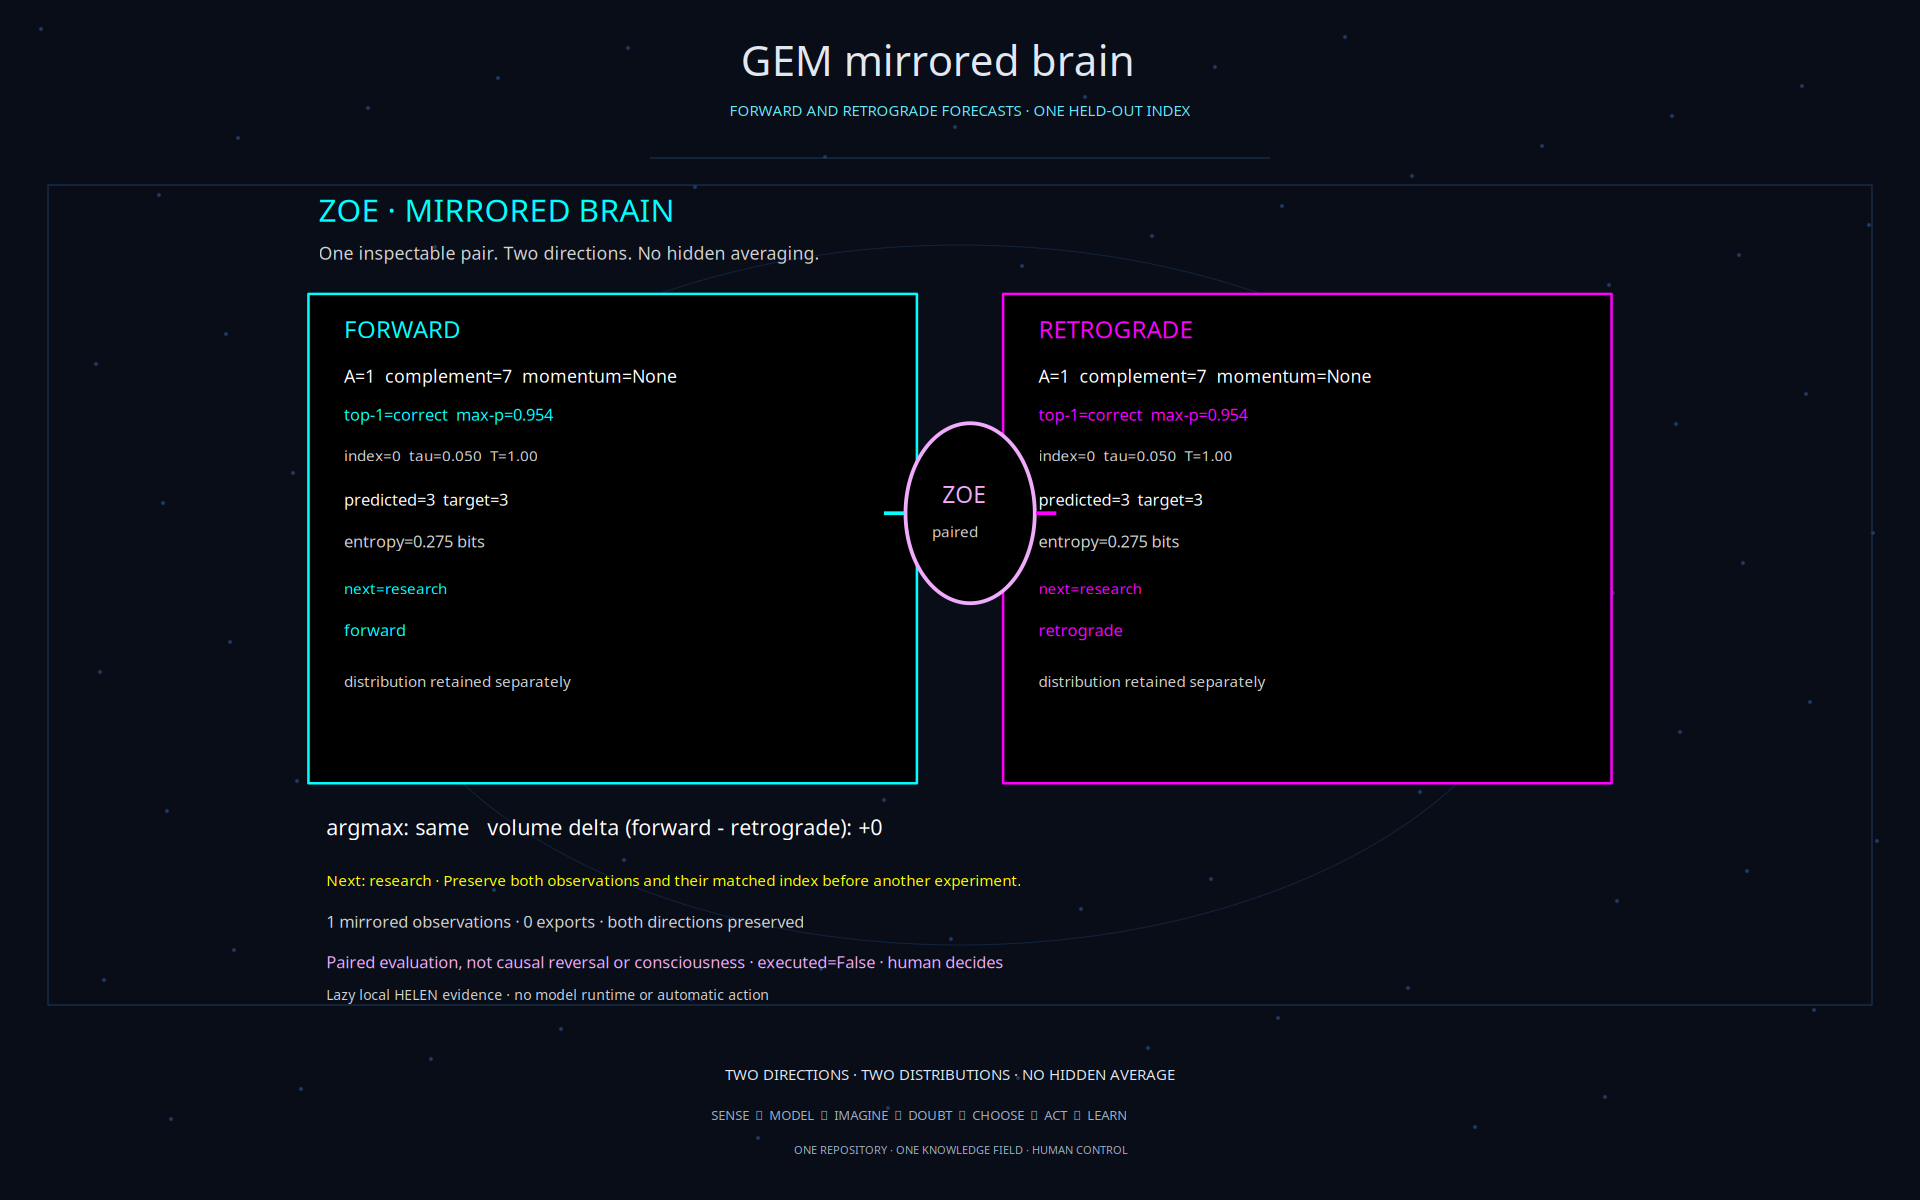
\includegraphics[width=\textwidth]{zoe-mirror.png}
\caption{A mirrored Zoe observation preserves two distributions at one index. Agreement and disagreement guide inspection only.}
\label{fig:mirror}
\end{figure}

The unified workbench exposes 17 operations: 13 original sections covering Bayesian updates, strict/adaptive/joint volume, forecast measurement, momentum, temperature, categorical sampling, Markov transitions, timing RMSE, Procrustes alignment, and inspection priority; causal-repertoire normalization; q-arrow annotation; two-way records; and mirrored observation. Independent expected-result checks passed for all 17. These checks verify calculations and software behavior, not empirical IIT, universal future prediction, or autonomous action.
